
\documentclass[a4paper,12pt]{article}

% بسته‌های ریاضی برای معادلات و نمادهای پیشرفته
\usepackage{amsmath, amssymb, amstext, siunitx}

% بسته رنگ برای استفاده از رنگ در متن یا محیط‌ها
\usepackage{xcolor}

% بسته گرافیک برای درج تصاویر
\usepackage{graphicx}

% تنظیمات حاشیه صفحه
\usepackage{geometry}

% بسته لینک‌دهی (هایپرلینک‌ها)
\usepackage{hyperref}

% بسته صفحه‌آرایی برای تنظیم هدر و فوتر
\usepackage{fancyhdr}

% بسته xepersian برای پشتیبانی از زبان فارسی با XeLaTeX
\usepackage{xepersian}

% تعیین فونت فارسی (فایل فونت باید موجود باشد یا در سیستم نصب باشد)
\settextfont{B Nazanin}

% تنظیم اندازه حاشیه‌ها از هر طرف برابر با 1 اینچ
\geometry{
	left=1.5cm,
	right=1.5cm,
	top=2.5cm,
	bottom=2.5cm
}

% تنظیم سبک fancy برای سربرگ و پاورقی
\pagestyle{fancy}

% سمت چپ هدر: مشخص‌کننده سری تمرین و نام درس
\lhead{تمرین سری چهارم درس فیزیک مدرن}

% وسط هدر: نام دانشکده
\chead{دانشکده فیزیک دانشگاه صنعتی خواجه نصیرالدین طوسی}

% سمت راست هدر: تاریخ روز به‌صورت خودکار
\rhead{\today}

% پایین صفحه: شماره صفحه
\cfoot{\thepage}

% شروع سند
\begin{document}
	
	% صفحه عنوان (بدون هدر و فوتر)
	\thispagestyle{empty}
	\begin{center}
		% لوگوی دانشگاه (در صورت وجود فایل تصویر در مسیر مشخص شده)
		
\includegraphics[width=0.5\textwidth]{../../../images/image-E_4/image-1.png} \\[10pt]
		% عنوان سند
		\textbf{\LARGE عنوان: تمرین سری چهارم}\\[20pt]
		
		% نیم‌سال تحصیلی
		\textbf{\LARGE نیم‌سال تحصیلی: ۴۰۴۲ }\\[10pt]
		
		% نام مدرس درس
		\textbf{\Large مدرس: دکتر تقی‌زاده}\\[10pt]
		
		% مبحث تمرین
		\textbf{\Large مبحث تمرین:فصل سوم }\\[10pt]
		
		% مهلت تحویل تمرین
		\textbf{\Large مهلت تحویل: ۲۹ خرداد}
	\end{center}
	
	% صفحه جدید برای ادامه سند
	\newpage
	
	% ایجاد فهرست مطالب به‌صورت خودکار (براساس \section ها)
	\tableofcontents
	\newpage
	
	\section{سوال اول}
	با نوشتن جزییات کامل ریاضی روابط کامپتون اثبات کنید. 
	\section{سوال دوم}
	
	در یک آزمایش تداخل دوشکاف یانگ، از نور سدیم با طول موج
	\(
	\lambda = 589.0\,\mathrm{nm}
	\)
	استفاده می‌شود. فاصله بین دو شکاف برابر
	\(
	1.25\,\mathrm{mm}
	\)
	و فاصله پرده از شکاف‌ها برابر
	\(
	2.604\,\mathrm{m}
	\)
	است.
	
	با استفاده از روابط تداخل نور، فاصله بین دو بیشینه متوالی (نوارهای روشن مجاور) روی پرده را محاسبه کنید.
	\section{سوال سوم}
	
	تکانه ذرات زير را محاسبه کنيد:
	
	\begin{enumerate}
		\item[(الف)] يک فوتون گاما با انرژي
		\[
		10.0\,\mathrm{MeV}
		\]
		
		\item[(ب)] يک فوتون پرتو ايکس با انرژي
		\[
		25\,\mathrm{keV}
		\]
		
		\item[(پ)] يک فوتون فروسرخ با طول موج
		\[
		1.0\,\mu\mathrm{m}
		\]
		
		\item[(ت)] يک فوتون امواج راديويي با فرکانس
		\[
		150\,\mathrm{MHz}
		\]
	\end{enumerate}
	
	در هر مورد، تکانه را هم بر حسب $\mathrm{kg \cdot m/s}$ و هم بر حسب $\mathrm{eV}/c$ بيان‌کنيد.
\section{سوال چهارم}

نوري با طول موج \(304.2\,\mathrm{nm}\) به سطح يک فلز تابيده مي شود. طول موج آستانه اين فلز برابر \(352.8\,\mathrm{nm}\) است.

با استفاده از معادله اثر فوتوالکتريک اينشتين، پتانسيل توقف \lr{(Stopping Potential)} را محاسبه کنيد.
\section{سوال پنجم}

(الف) با فرض اين که خورشيد مانند يک منبع گرمايي ايده آل با دماي \(6000\,\mathrm{K}\) تابش مي کند، شدت تابش خورشيدي در بازه طول موج \(530.0\,\mathrm{nm}\) تا \(532.0\,\mathrm{nm}\) را محاسبه کنيد.

(ب) اين بازه چه کسري از کل تابش خورشيدي را تشکيل مي دهد؟
	
	\section{سوال ششم}
	
	يک حفره در دماي \(1750\,\mathrm{K}\) نگه داشته شده است. انرژي با چه نرخي از داخل حفره از طريق سوراخي در ديواره آن با قطر \(1.24\,\mathrm{mm}\) خارج مي شود؟
	\section{سوال هفتم}
	
	پرتو هاي گاما با انرژي بالا مي توانند از طريق پراکندگي کامپتون از محيط اطراف به يک آشکارساز برسند، همان طور که در شکل زیر نشان داده شده است. اين اثر با نام \lr{back-scattering} شناخته مي شود.
	
	نشان دهيد که وقتي \(E \gg m_e c^2\) باشد، فوتون پراکنده شده در حالت بازپراکندگي (زاويه پراکندگي نزديک به \(180^\circ\)) داراي انرژي تقريبا \(0.25\,\mathrm{MeV}\) است و اين مقدار تقريبا مستقل از انرژي فوتون اوليه است.
	\begin{figure}[h]
		\centering
		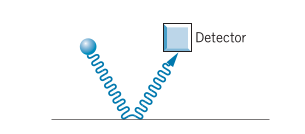
\includegraphics[width=0.5\textwidth]{../../../images/image-E_4/image-2.png}
		\caption{ \lr{back-scattering} }
	\end{figure}
	\section{سوال هشتم}
	
	ماهواره \lr{WMAP} که در سال 2001 پرتاب شد، تابش زمینه کیهانی \lr{(Cosmic Microwave Background Radiation)} را بررسی کرد و توانست نوسانات بسیار کوچک دما در نواحی مختلف این تابش را اندازه گیری کند. این نوسانات دمایی متناظر با نواحی با چگالی زیاد و کم در جهان اولیه هستند.
	
	این ماهواره توانست اختلاف دمایی برابر \(2 \times 10^{-5}\,\mathrm{K}\) را در دمای متوسط \(2.7250\,\mathrm{K}\) اندازه گیری کند.
	
	در طول موج بیشینه تابش، اختلاف شدت تابش به ازای واحد بازه طول موج بین نواحی "داغ" و "سرد" را محاسبه کنید.
	
	\section{سوال امتیازی اول}
	
	ماهواره \lr{COBE} در سال 1989 برای مطالعه تابش زمینه کیهانی و اندازه گیری دمای آن پرتاب شد. با اندازه گیری در طول موج های مختلف، پژوهشگران نشان دادند که این تابش دقیقا از توزیع طیفی مورد انتظار برای یک جسم سیاه پیروی می کند.
	
	در طول موج \(0.133\,\mathrm{cm}\)، شدت تابشی برابر \(1.440 \times 10^{-7}\,\mathrm{W/m^2}\) در بازه طول موج \(0.00833\,\mathrm{cm}\) اندازه گیری شده است.
	
	دمای تابش جسم سیاه متناظر با این داده ها را محاسبه کنید.
	\section{سوال امتیازی دوم}
	
	
	\begin{enumerate}
		
		\item[(الف)] نشان دهید در توصیف کلاسیک از توزیع انرژی نوسانگرهای دیواره حفره، اگر انرژی های مجاز به صورت \(E_n = n\varepsilon\) در نظر گرفته شوند، آنگاه جمع تعداد کل نوسانگرها روی همه حالت ها برابر \(N\) خواهد بود.
		
		\item[(ب)] نشان دهید در حد کلاسیک، انرژی متوسط هر نوسانگر برابر است با
		\[
		E_{avg} = kT
		\]
		
	\end{enumerate}
	
	\textbf{نوسانگرهای دیواره حفره پلانک}
	
	اگر توزیع ماکسول بولتزمن برای نوسانگرها به صورت
	\[
	N_n = A e^{-E_n/kT}
	\]
	در نظر گرفته شود و انرژی ها به صورت \(E_n = n\varepsilon\) باشند:
	
	\begin{enumerate}
		\item[(الف)] با شرط نرمال سازی
		\[
		\sum_{n=0}^{\infty} N_n = N
		\]
		نشان دهید ثابت نرمال سازی برابر است با
		\[
		A = N\left(1 - e^{-\varepsilon/kT}\right)
		\]
		
		(راهنما: از سری هندسی استفاده کنید.)
		
		\item[(ب)] با مشتق گیری از رابطه سری هندسی، نشان دهید
		\[
		\sum_{n=0}^{\infty} n x^n = \frac{x}{(1-x)^2}
		\]
		
		\item[(ج)] با استفاده از نتیجه قسمت قبل، نشان دهید انرژی متوسط نوسانگرها برابر است با
		\[
		E_{avg} = \frac{\varepsilon}{e^{\varepsilon/kT} - 1}
		\]
		
		\item[(د)] حدهای زیر را بررسی کنید:
		\[
		E_{avg} \approx kT \quad (\varepsilon \ll kT), \qquad E_{avg} \to 0 \quad (\varepsilon \gg kT)
		\]
		
		\item[(ه)] با بررسی شرط بیشینه شدن شدت تابش طیفی \(I(\lambda)\)، نشان دهید قانون جابجایی وین به دست می آید.
		
	\end{enumerate}
	
	\vspace{6pt}
	
	با انتگرال گیری از رابطه طیفی پلانک برای تابش جسم سیاه، توان کل تابش را به صورت زیر به دست آورید:
	\[
	I = \int_0^\infty I(\lambda)\, d\lambda
	\]
	
	و با استفاده از انتگرال استاندارد
	\[
	\int_0^\infty \frac{x^3}{e^x - 1} dx = \frac{\pi^4}{15}
	\]
	
	نشان دهید قانون استفان–بولتزمن به صورت
	\[
	I = \sigma T^4
	\]
	به دست می آید.
	
\end{document}